%!TEX root = ../thesis.tex
\chapter{Experiments}\label{chap:Experiments}
The amount of experiments, data and visualizations created in this project are more than a dedicated reader is confortable reading in one single pass. For this reason, the experiments and results in this chapter first presented with a simple example, the EmoLex. This example will guide the reader through the methodology to analyze the datasets, and introduce the intuitions presented through simpler visualizations with lesser data. With this intuitions in mind, the results of the other datasets, and language models are presented. In this way, the EmoLex works not only as an introduction to the methodology and results, but also as a lax baseline.

\section{EmoLex}\label{sec:EmoLex}
As an introductory experiment, EmoLex has been embedded into the abstract vector representation of the GloVe language model. This model was selected due to its one-to-one relation between word and embedding, and it's context indepedence. This means that a word will get one single embedding no matter what other words apear next to it. This in comparison to BERT, where the embedding of a single word deppends on the tokens, words, and sentences that come with it. The EmoLex has single words related to emotions, so it must be noted that this experiment and it's results relate to word embedding, and not sentence embedding.

\subsection{Correlational Analysis}
A correlational analysis answers the question of how much does every dimension of the language model relates to every emotion. The result of this model is a correlation matrix where every element of that matrix is a number between -1 and 1.
In the case of the EmoLex, abstracted into the GloVe laguage model, it is a $8x300$ matrix, where the rows correspond to the 8 emotions represented in the EmoLex. This matrix is visualized in Figure~\ref{fig:cor_emolex_GloVe}. The plot shown in this figure is called a clustermap. It was created with pythons Seaborn library, and consists of two parts:

The main part is the visualization of the matrix. In this visualization, every number of the matrix is given a color from a range of colors shown in the colorbar. The range is automatically set from the maximum and minimum number in the matrix. This allows to see paterns in the releationships between the vector space dimentions and the emotions, if there are any.

The second visualization of this plot is the left dendrogram. A dendrogram is the visualization of a clustering structure. This clustering is done through a nearest neighbor algorithm, using euclidian distance.

A correlational plot is used here to analyze the deviation of the distribution of the representation of variables in the different dimensions of the vector space. In this case, there are 8 variables. A uniformely random distribution of the representation would yield a correlation of 0.125. Thus a correlation of  0.125 or lower is considered random. In our baseline reference by Hollis et al.~\cite{hollis2016principals}, where they analyzed 9 variables the minimum significant correlation reported was 0.35. This is more than three times the correlation of a uniformely random distribution: 0.111\underline{1}

\begin{figure}[H]
  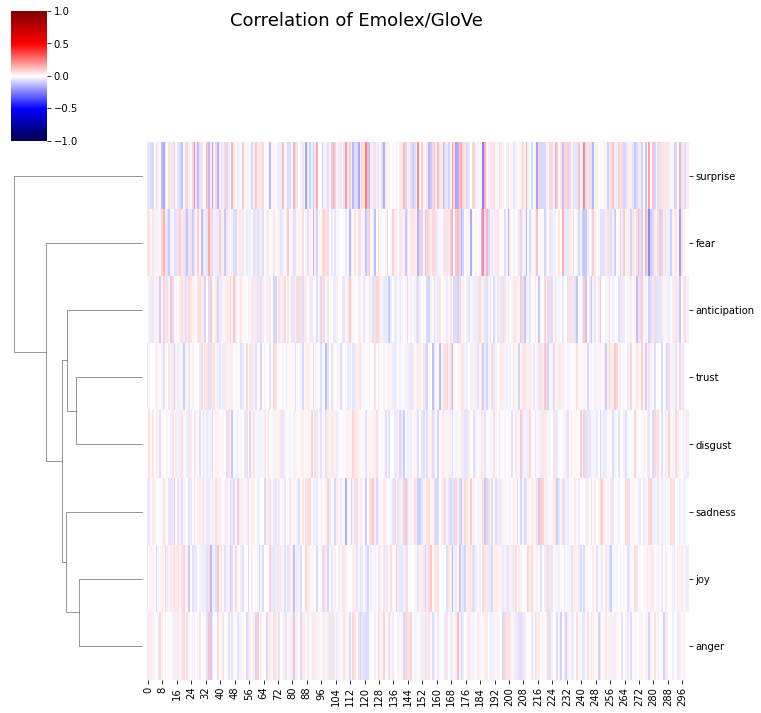
\includegraphics[width=\textwidth]{plots/emolex/cor_emolex_GloVe}
  \centering
  \caption{EmoLex Correlation Plot}
\end{figure}\label{fig:cor_emolex_GloVe}

In Figure~\ref{fig:cor_emolex_GloVe} it can be observed that represented by the GloVe model, the words contained in the EmoLex are uniformely distributed through the dimensions. The maximum correlation is 0.251, between the emotion \"Trust\" and dimension 121 of the model. Although this is double the correlation that could be found throgh chance, it does not satisfy the baseline condition, and thus, we cannot consider that there is a linear correlation between the emotions of the EmoLex, and the dimensonal representation of the Language Model.

The corresponding clustering algorithm shows that through their vectorial representation, the two most related emotions are joy and anger. This does not comply with the findings of dichotomical emotions, fitting into a valence model, as shown in the 2016 study~\cite{barradas2016thesis}.

These two results are enough to reject the hypotesis that there is a linear correlation between the emotions in the EmoLex and the vectorial representation of the GloVe model.


A further correlational study can be done solely to the labels of the EmoLex. This is here called an Emotion-to-Emotion correlation, and it's obtained through the self-correlation matrix of the one-hot-encoding of the EmoLex emotion labels. The clustermap of said matrix can be seen on Figure~\ref{fig:cor_emolex_GloVe_e_e}. An organic distribution of these would show the expected hierarchical clustering between positive and negative emotions. This plot, although labeled as related to the GloVe, is independant from the language model, since it only looks at the labels, but the name has been kept for consistency.

\begin{figure}[H]
  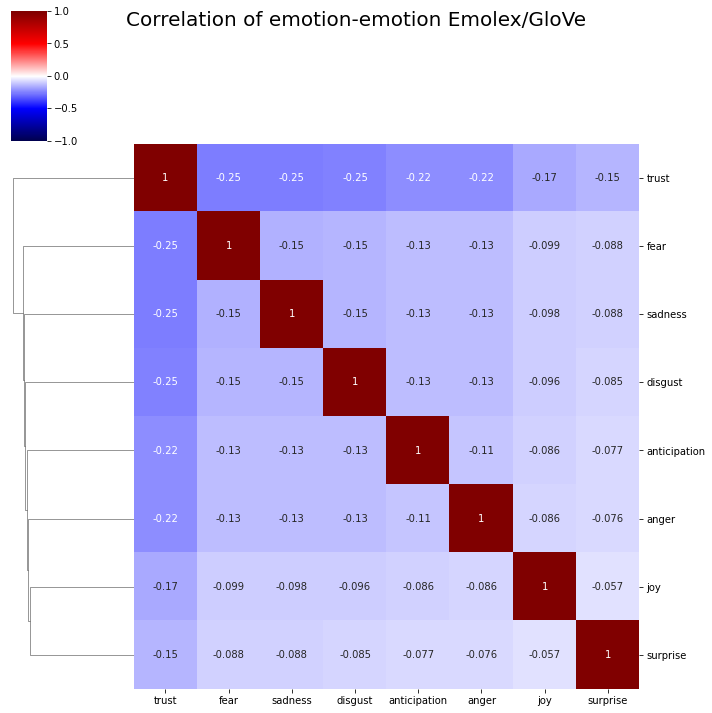
\includegraphics[width=1\textwidth]{plots/emolex/cor_emolex_GloVe_e_e}
  \centering
  \caption{EmoLex Correlation Plot}
\end{figure}\label{fig:cor_emolex_GloVe_e_e}

The EmoLex is not an organic corpus, and thus the labels do not represent the hierarchical clustering shown in the 2016 study~\cite{barradas2016thesis}. Instead the emotions are uniformely distributed. This is expected for a lexicon.

\subsection{PCA}
By maximizing the ammount of information represented by the first components through a linear transformation of the data, a PCA analysis provides a perspective on the representation of variables in the model that cannot be seen through a simple correlation.

By visualizing a scatter plot of the first components or PCA dimensions, if there is a linear separation between the labels it can be visualized. Even in the case of data that is not linearly separable, a gradient of the distribution of the data could indicate the existance of a structure.

\begin{figure}[H]
  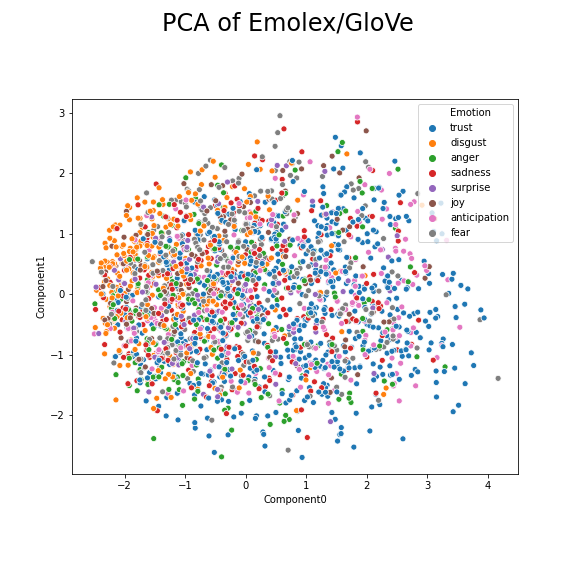
\includegraphics[width=1\textwidth]{plots/emolex/pca_scat_emolex_glove}
  \centering
  \caption{EmoLex Scatter plot of PCA}
\end{figure}\label{fig:pca_scat_emolex_glove}

In Figure~\ref{fig:pca_scat_emolex_glove} we can see the scatter plot of the words of the EmoLex, projected on to the first two components of the PCA transformation. Here we can observe, that the words labeled with the emotion disgust are mostly centered to the top-left of the plot. Although this might seem like the indication of a structure, we cannot certantly point at it. This plot is useful for visualizing linear separation, but that linear separation does not show in this case. To be able to visualize what the PCA transformation does to the vector space, the correlation matrix is shown next.

The correlation matrix shown next is the same type of visualization as the one in Figure~\ref{fig:cor_emolex_GloVe}, but this is done to the transformed dataset. This means that the x-axis shows the number of the component instead of the dimension of the language model.

\begin{figure}[H]
  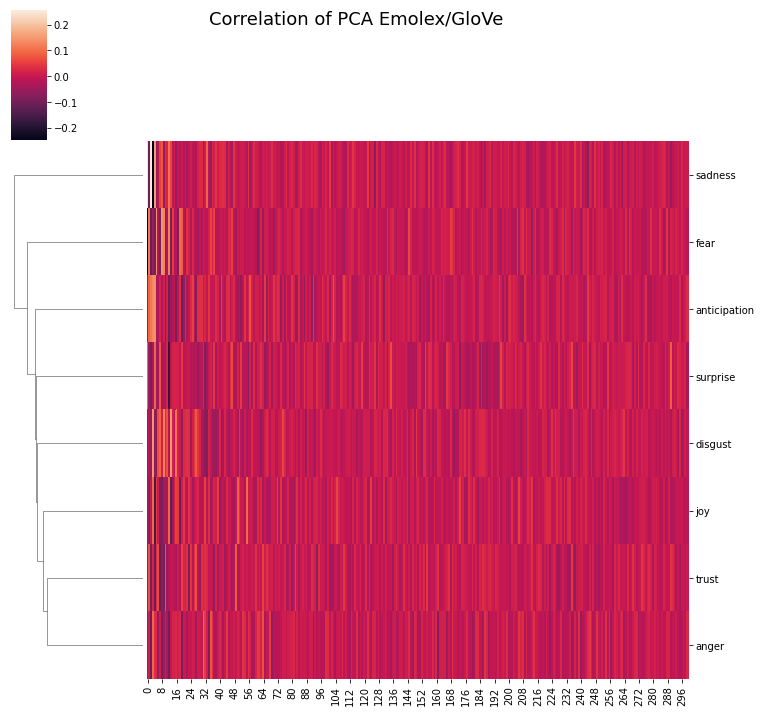
\includegraphics[width=1\textwidth]{plots/emolex/pca_cor_emolex_glove}
  \centering
  \caption{EmoLex Correlation of all PCA components}
\end{figure}\label{fig:pca_cor_emolex_glove}

By plotting the correlation matrix of the PCA transformation of the EmoLex, we can observe that most of the variability is concentrated on the first components. Still in this case, the maximum correlation is 0.2567, barely higher than on the linear correlation. The hierarchical clustering shows no precence of a valence-correspondant clustering.

Considering that the PCA is a linear transformation we do not expect to see better correlations between the model dimentions, and the concepts, but a dense representation that does not require looking at all dimensions. For this reason, when looking at PCA correlations, only the first eight dimensions will be shown. Eight is an arbitrary number that allows a square correlation matrix, since it's the same number of emotions for this dataset.

\begin{figure}[H]
  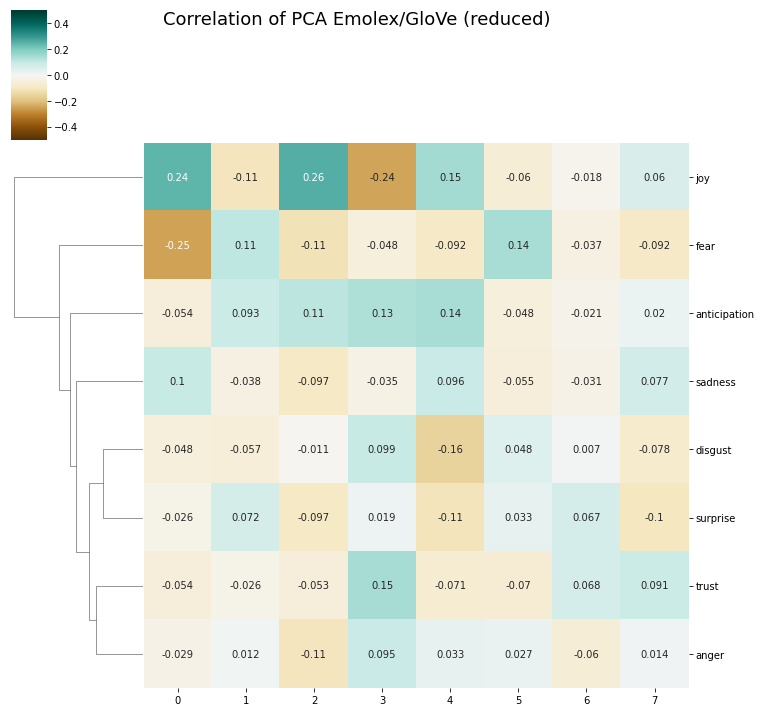
\includegraphics[width=1\textwidth]{plots/emolex/pca_cor_emolex_glove_min}
  \centering
  \caption{EmoLex Correlation of first PCA components}
\end{figure}\label{fig:pca_cor_emolex_glove_min}

Figure~\ref{fig:pca_cor_emolex_glove_min} shows the first 8 dimentions of the PCA transformation for this model and dataset. A different color scheme has been selected to easily identify between the linear correlation visualization, and the PCA-transformed correlations. This is the exact same data as the one used to create Figure~\ref{fig:pca_cor_emolex_glove}, but since only the most information-dense dimensions are being shown, the hierarchical clustering is much different. Here we can observe that what had no apparent structure now seems to cluster disgust with surprise, and trust with anger. By observing only the first component, we can see that if it activates, we can expect that the emotion Joy is not expressed in the embedding, with a 24\% probability, and that fear is not expressed with 25\% probability. This results are not very concise, but this is expected due to the artificial nature of the dataset, and the subjectivity of the concepts. In the expreiments section of this chapter we aim at describing how much of that variability is due to the subjectivity of the concept.

\subsection{TSNE}
Through this, non-linear visualization algorithm we can plot a scatter that will concentrate the maximum variability possible on two dimensions. The result is the plot on Figure~\ref{fig:tsne_scat_emolex_glove}.

\begin{figure}[H]
  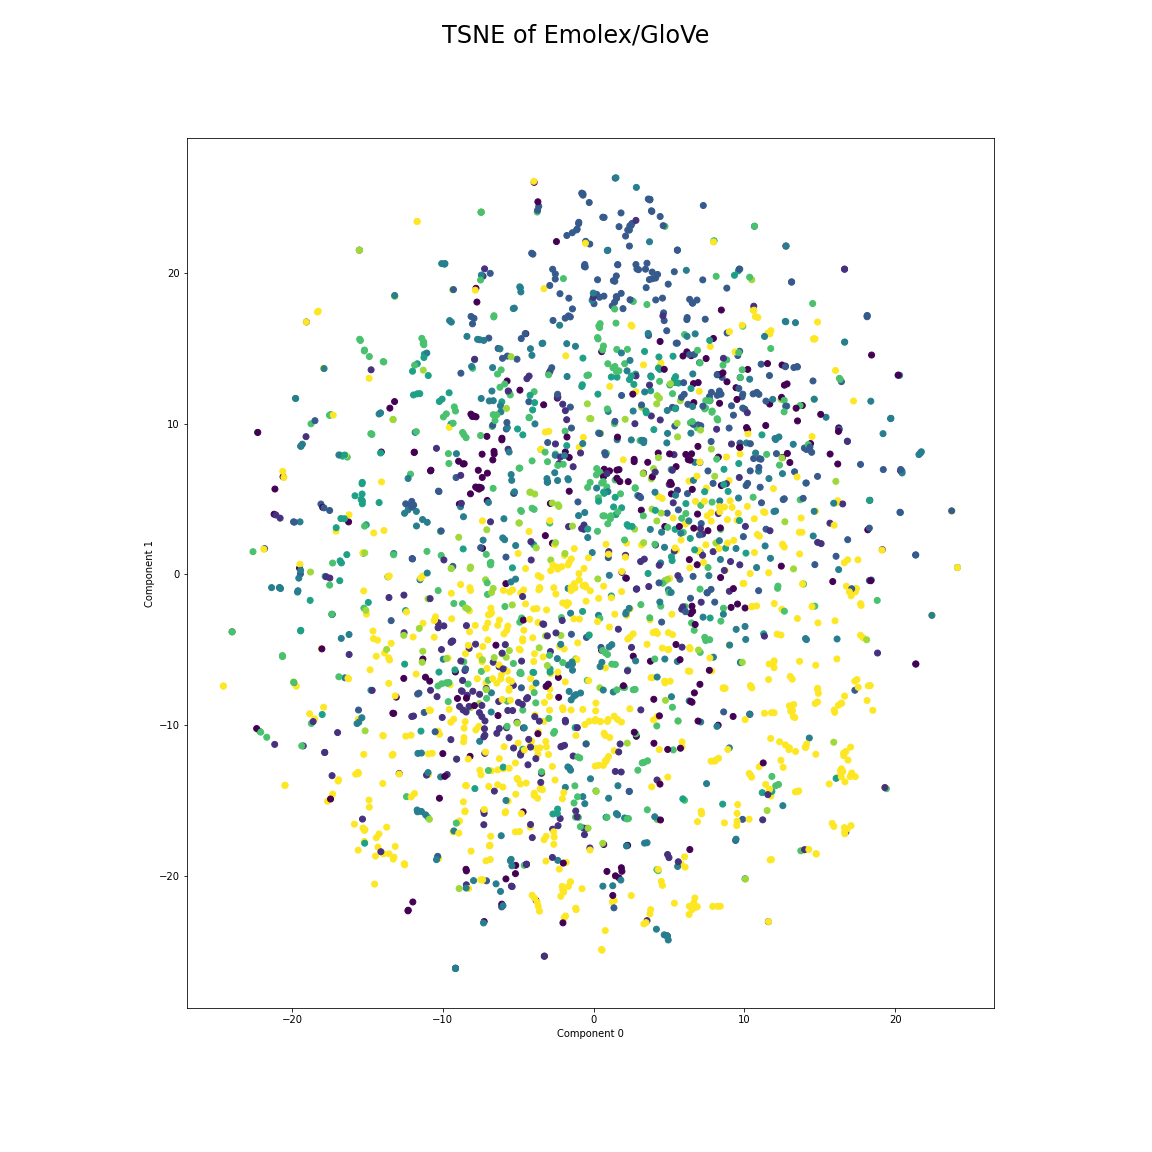
\includegraphics[width=1\textwidth]{plots/emolex/tsne_scat_emolex_glove}
  \centering
  \caption{EmoLex Scatter plot of TSNE}
\end{figure}\label{fig:tsne_scat_emolex_glove}

In this plot we can observe that two major distribution centers are created: one on the top of the plot and one on the bottom. The two groups are represented by two emotions: trust and disgust. These two are indeed polar opposites on the Plutchik model.

Within the these two groups, we can also observe sub-clusters. A further analysis of the plot has been done with the help of a bokeh interactive plot, present in html format in the plots folder of the repository. Here we can read the words in the subcusters.

One of the subclusters with the trust label is the one formed by the words: aposite, apostolic, chapland, vicar, episcopal, parish, deacon, ordained, priest, congregation. The subcluster also contains the word reverend, labeled with the emotion joy, and is very close to the subcluster with the words convent, nun, monk, abbot, and cannons, labeled with trust, and mystic, labeled with surprise.

With this example we can comment on what we expect to see in further experiments. Subclusters are formed by words that have semantic relationship, as it is expected from a functional language model, and the emotions labeled on to that word are an expression of the context of the person labeling the word, more than the intrinsic emotion of the word. This is conformant with the theory of constructed emotions.

These subclusters form an important part of the analysis, and have therefore been given a name: \"semantic islands\". A semantic island is a cluster of datapoints that have a semantic relationship.

As it is expected from a non-organic dataset, the structure to be found seems artificial. The distribution of the labels and words is uniform, and no conclusion must be drawn form it to apply to general language. Nontheless, the visualization of the EmoLex as a dataset lets us develop the beggining of an intuition, and a technique as of how to approach this problem. In the following section, the same methodology will be followed to analyze the selected datasets and models.



\section{Results}\label{sec:Results}

The following results are separated into three: The correlation analisis, the PCA, or linear transformation, and the TSNE, or non-linear transformation.

%TODO: talk about the specifics of crowdflower

%TODO: expand

%===============================================================================
\subsection{Correlation Analysis}\label{sub:Correlation Analysis}
A linear correlation is now compared between the four forementioned language models. The results that best abstract the specifics of this dataset are those of the FastText model, since it has been trained specifically for this dataset. This is our baseline, and thus will be presented first:


\subsubsection{FastText}
With the FastText model, the maximum correlation was shown in the supervised approach, with 33.45\% correlation between the hapiness emotion, and it's third dimension. The visualization of said model is shown in Figure~\ref{fig:cor_CrowdFlower_FastText}.

\begin{figure}[H]
  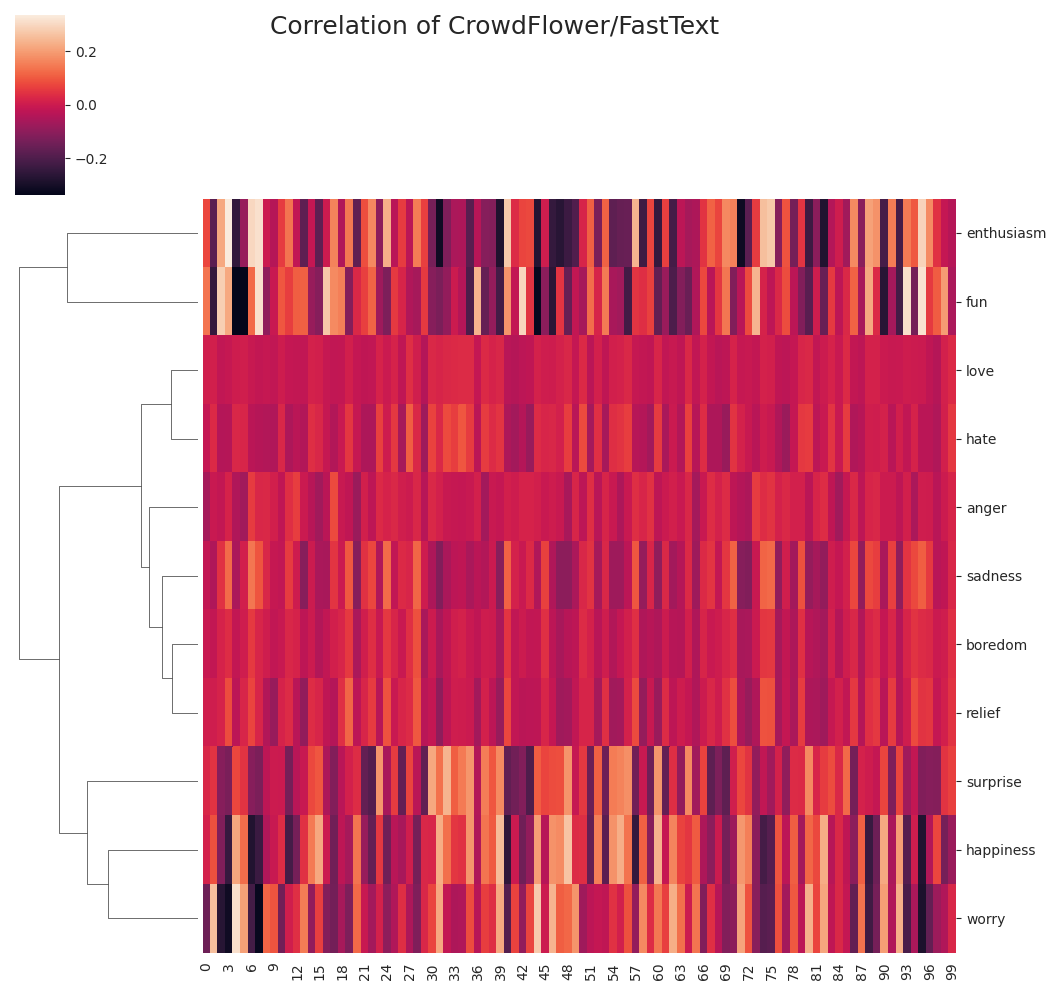
\includegraphics[width=1\textwidth]{plots/cor/cor_CrowdFlower_FastText}
  \centering
  \caption{Correlation plot for FastText}
\end{figure}\label{fig:cor_CrowdFlower_FastText}

A hierarchical structure of the concepts can also be observed, with two main groups: fun and enthusiasm in one, with a high activation of all dimensions (be it possitive or negative), and the rest on a second group. The latter can be subdivided into two. The first group contains emotions of surprise, happiness, and worry, while the second one contains the rest of the emotions with very little activation.

An interesting observation is that love and hate have been clustered together, even if the activation of the vector space is very reduced.

\subsubsection{Word2Vec}
Word2Vec is the first pre-trained model to be reviewed. This model has been observed to contain an abstraction of valence, and it is thus expected to show it. Hollis et al. report that 208 dimensions out of the 300 dimensions of te model correlate with the concept of valence. They unfortunately do not mention how much the dimensions correlote~\cite{hollis2016principals}. In this case, the model's maximum correlation was between the happiness concept, and it's 43th dimension, with 11.94\%. This is means that most of the dimensions did not correlate significatntly with the concepts we are exploring, since the random threshold is 9.09\%, and the maximum correlation found barely surpases that, with most of them under the treshold.

\begin{figure}[H]
  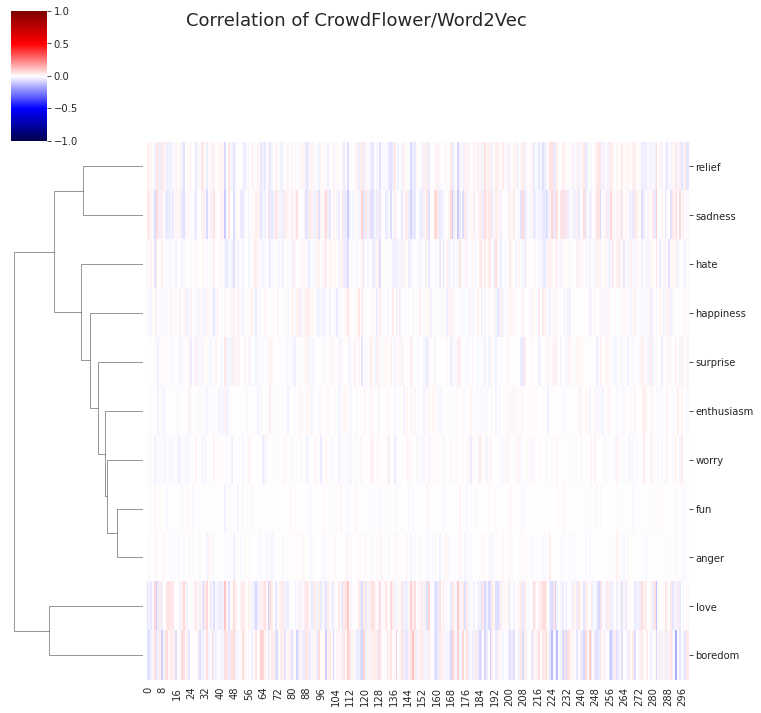
\includegraphics[width=1\textwidth]{plots/cor/cor_CrowdFlower_Word2Vec}
  \centering
  \caption{Correlation plot for Word2Vec}
\end{figure}\label{fig:cor_CrowdFlower_Word2Vec}

Figure~\ref{fig:cor_CrowdFlower_Word2Vec} shows the mentioned correlations. At first sight, it might seem that the clustering is similar to the one shown with FastText, with two main groups, one of which is again separated into two, but the emotions clustered are not the same. Clustered together are love and boredom, releif and sadnes, and fun and anger. These are neither opposites, nor subsets of a valence side.

\subsubsection{GloVe}
The GloVe model presents a higher complexity than the Word2Vec. Thus, better results are expected. Here, the best correlation was 11.97 \%, between the worry concept, and the 164 dimension.This is again, barely above the random treshold.
\begin{figure}[H]
  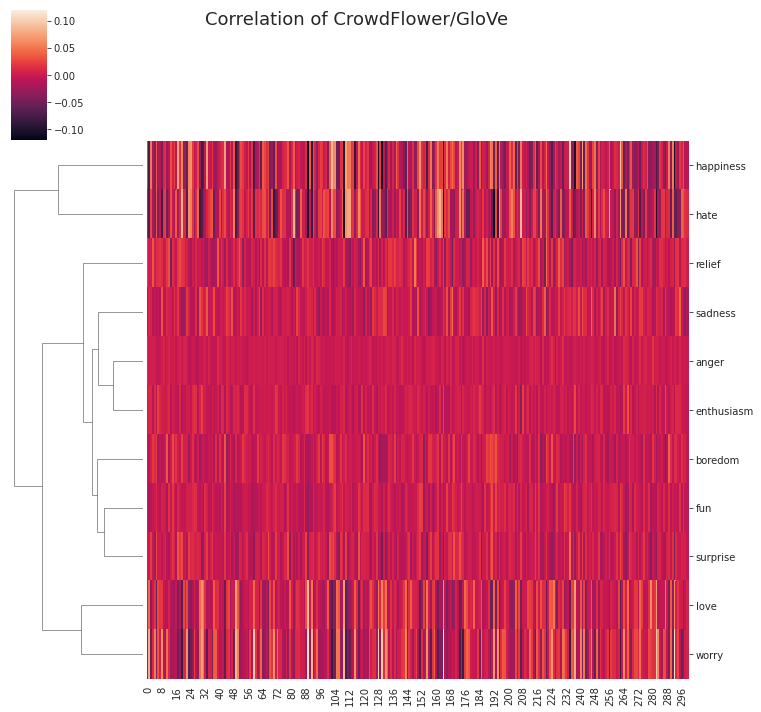
\includegraphics[width=1\textwidth]{plots/cor/cor_CrowdFlower_GloVe}
  \centering
  \caption{Correlation plot for GloVe}
\end{figure}\label{fig:cor_CrowdFlower_GloVe}
The clustering in Figure~\ref{fig:cor_CrowdFlower_GloVe} presents a similar structure, with different concepts as the last two models. Hate and happines form a group, while the rest separate into two subgroups: one with love and worry, and the rest of the concepts, with almost no correlation, in a single big cluster.

\subsubsection{BERT}
BERT is the most powerful language model used within this project. Still, it presented a maximum correlation of only 13.87\% between the love concept, and dimension 305. Although slightly better than the previous results, it is still within the treshold of random sampling.
\begin{figure}[H]
  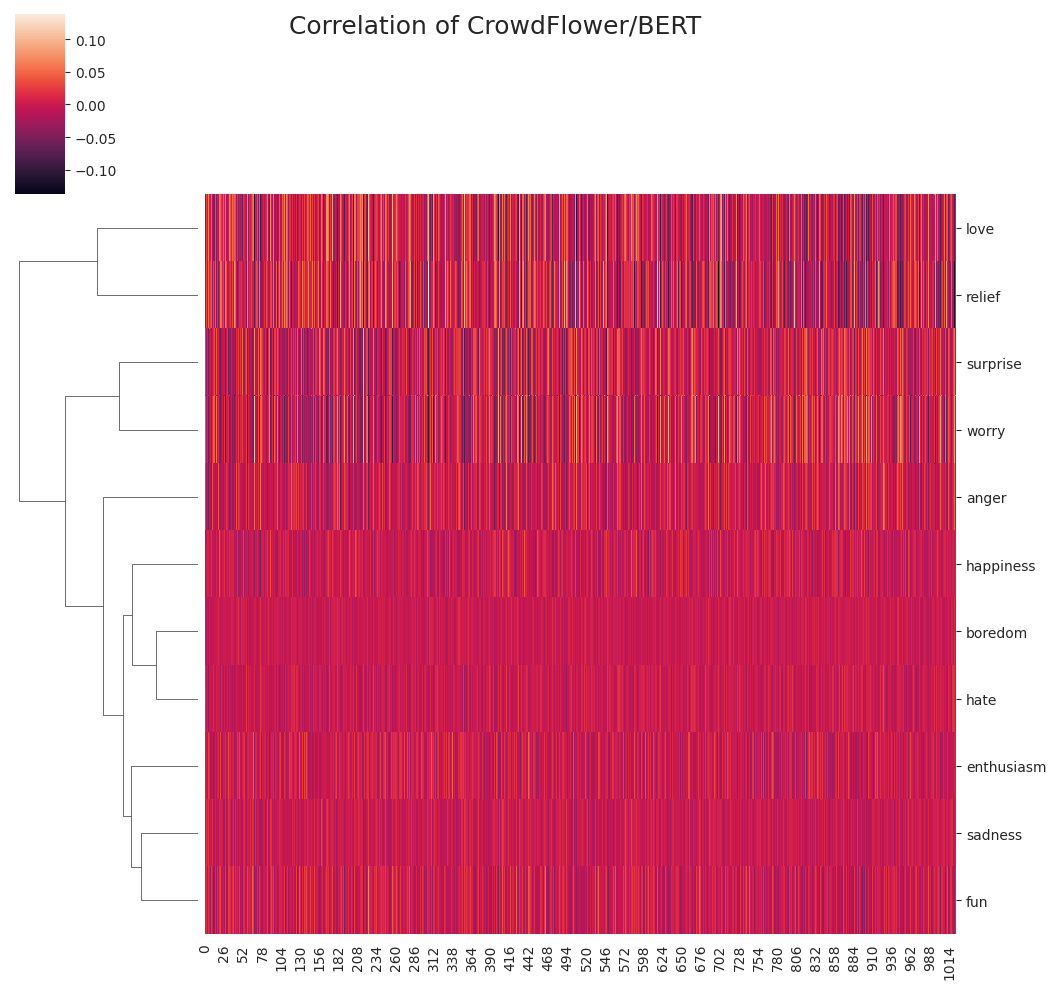
\includegraphics[width=1\textwidth]{plots/cor/cor_CrowdFlower_BERT}
  \centering
  \caption{Correlation plot for BERT}
\end{figure}\label{fig:cor_CrowdFlower_BERT}
On Figure~\ref{fig:cor_CrowdFlower_BERT}, we can observe that the concepts that most activate the latent dimensions in this model are love, relief, surprise, and worry. Love and Relief cluster into one group, Surprise and Worry in another. Not much structure can be observed, but sadness and fun did cluster into the less activated cluster.

\subsubsection{Analysis Discussion}
As we can see with these analysis, the linear interpretation of the dimensions of an embedded dataset, through a pre-trained language model does not provide consistent information about the representation of those concepts by the language model.


%===============================================================================
\subsection{Linear Transformation Analysis}\label{sub:Linear Transformation Analysis}
A linear transformation of the vector space generated by the laguage model can concentrate the information of said model on very little dimensions. This allows for a different analysis of the embedding of the concepts. For this analysis, we have selected the 11 top components of the PCA trasformation. This allows us to see the numeric values in the visualization.

\subsubsection{FastText}
The baseline FastText analysis shows that the mostly correlated model was the supervised model, shown in Figure~\ref{fig:pca_cor_CrowdFlower_FastText}. This shoed a maximum correlation of 36.85\% with the concept of hate. This is a slight improvement over the non-transformed analysis.
\begin{figure}[H]
  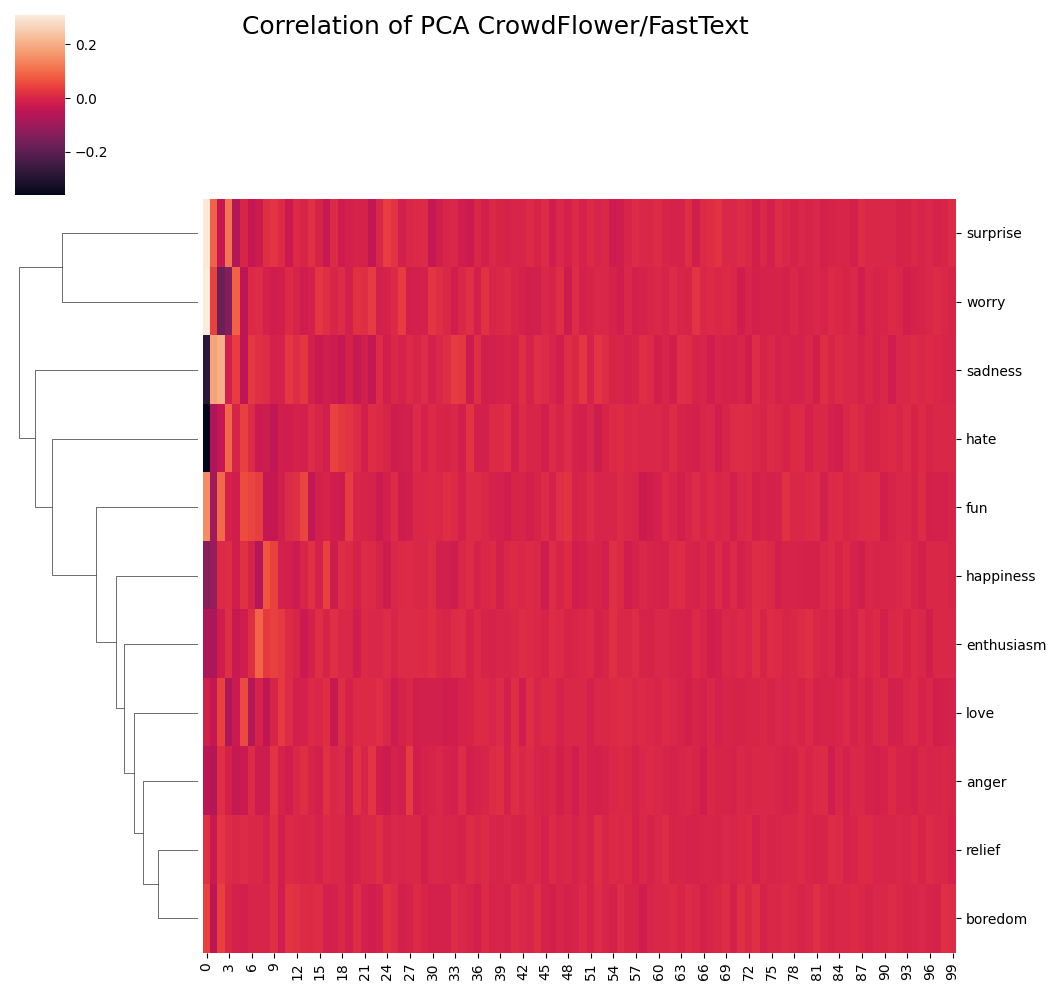
\includegraphics[width=1\textwidth]{plots/pca/pca_cor_CrowdFlower_FastText}
  \centering
  \caption{PCA Correlation plot for FastText}
\end{figure}\label{fig:pca_cor_CrowdFlower_FastText}
Figure~\ref{fig:pca_cor_CrowdFlower_FastText} shows that the first component of the transformation has a high positive correlation with the concepts of Surprise and Worry, while keeping a high negative correlation with Sadness and Hate. One grouping between Surprise and Worry is present, with the rest of the concepts in a second cluster.

\subsubsection{Word2Vec}
The transformation of the Wort2Vec representation presents the worst representation of concepts seen. The maximum correlation present is between the Love concept, and the second component.
\begin{figure}[H]
  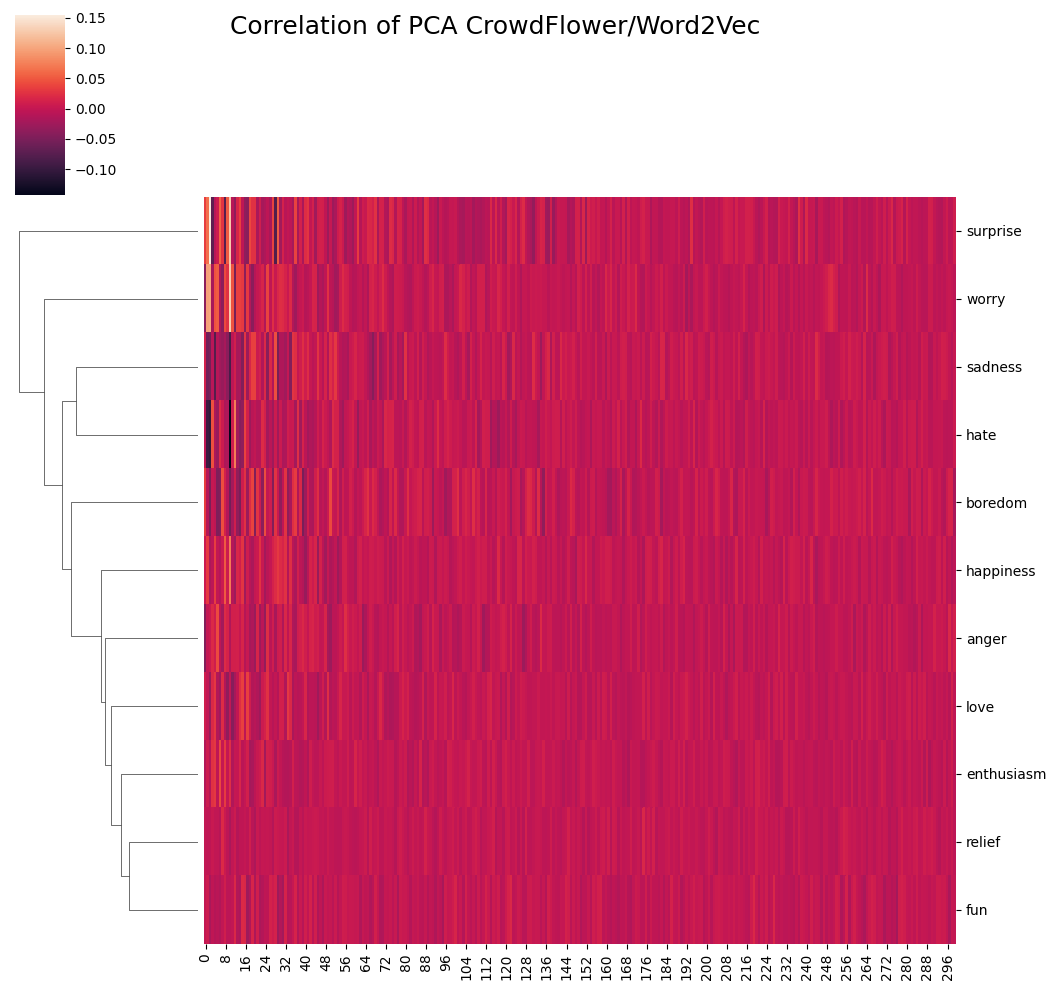
\includegraphics[width=1\textwidth]{plots/pca/pca_cor_CrowdFlower_Word2Vec}
  \centering
  \caption{PCA Correlation plot for Word2Vec}
\end{figure}\label{fig:pca_cor_CrowdFlower_Word2Vec}
Figure~\ref{fig:pca_cor_CrowdFlower_Word2Vec} shows the results of this analyzis. Here, with a very low correlation, sadness and hapiness have been clustered together, while relief and fun create the second most distinct group. The dichotomy of sadness and happiness is as expected from the baseline papers, but the correlation is much lower than if only valence is taken into account.
Another relevant grouping to mention is that of Anger and Worry. Although the direct correlations between the given concepts and the components of the transformed vector space are not statistically relevant, the clustering that can be done by analyzing these corresponds with that of parts of the Plutchik model, and accounts for dichotomy of emotions in a valence model of affect.

\subsubsection{GloVe}
The GloVe model shows a very low correlation, even worst that the Word2Vec model, which seems contradictory. The maximum correlation is 9.58\% lower than the threshold of random choice.
\begin{figure}[H]
  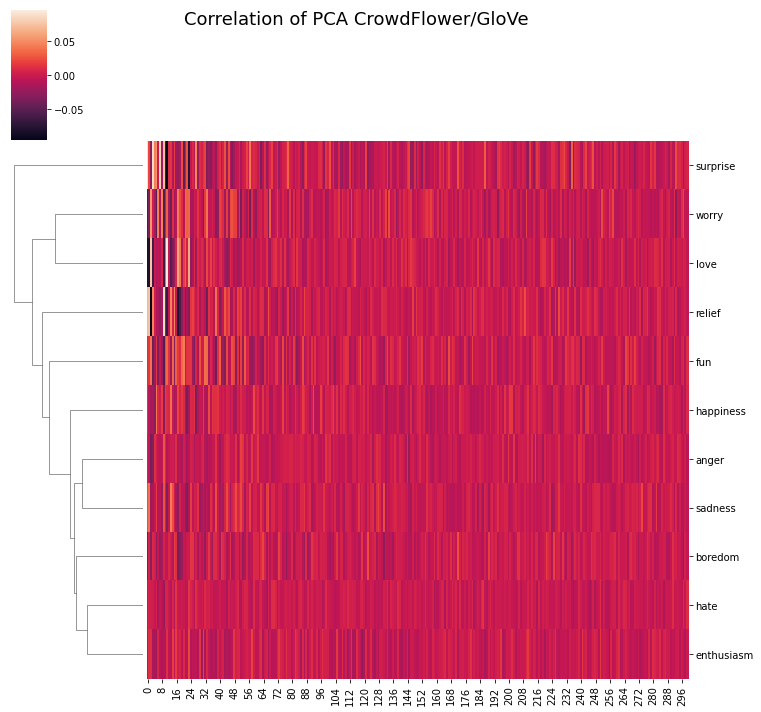
\includegraphics[width=1\textwidth]{plots/pca/pca_cor_CrowdFlower_GloVe}
  \centering
  \caption{PCA Correlation plot for GloVe}
\end{figure}\label{fig:pca_cor_CrowdFlower_GloVe}
Figure~\ref{fig:pca_cor_CrowdFlower_GloVe} shows how the low correlation of concepts and components of the PCA-transformed vector space yields no results that relate to emotion models. Even so, a three-group clustering is seen. This might indicate that this clustering is more related to the dataset, than to the language model.

\subsubsection{BERT}
The BERT model shows a maximum correlation of 10.28\% with between the component number 5 and the concept of Love. The correlations are not as high as expected, for the most powerful model in this project.
\begin{figure}[H]
  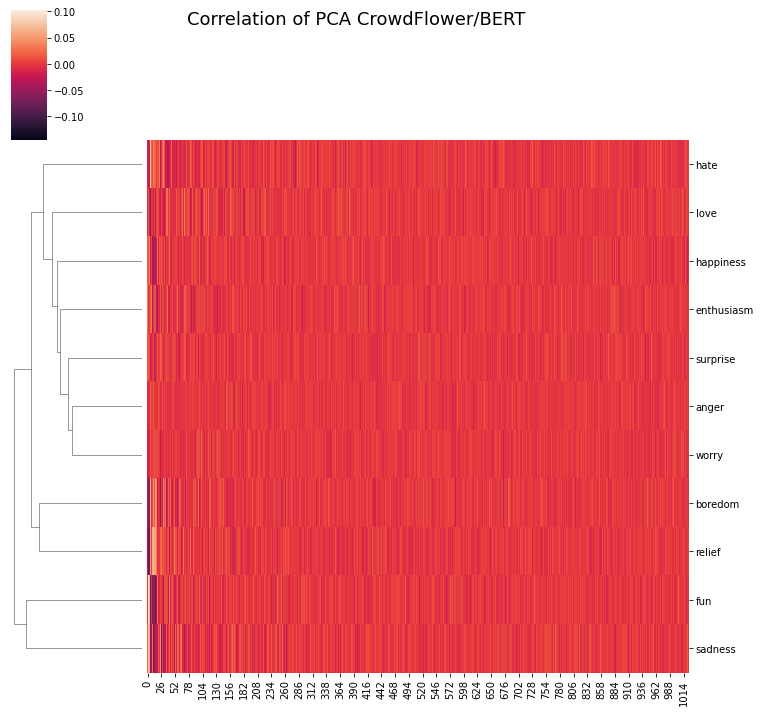
\includegraphics[width=1\textwidth]{plots/pca/pca_cor_CrowdFlower_BERT}
  \centering
  \caption{PCA Correlation plot for BERT}
\end{figure}\label{fig:pca_cor_CrowdFlower_BERT}
Figure~\ref{fig:pca_cor_CrowdFlower_BERT} shows how the results don't seem to be as densely populated by high correlations. This could be due to the high dimensionality of the model. With this PCA transformation 1024 dimensions are being reduced down to 10, which in comparison with the other models, is a much bigger reduction. No clustering seems relevant, when compared with emotion models.

\subsubsection{Analysis Discussion}
As mentioned before, a dimensionality reduction implies that some information will be lost by the model. If the information captured was already low, and the number of dimensions is significantly reduced, the results can end up being worst than random guess.

%===============================================================================
\subsection{Non-linear Transformation Analysis}\label{sub:Non-linear Transformation Analysis}
The TSNE non-linear dimensionality reduction allows for two-dimensional scatter plots that maximize the distance between groups in a dataset. A point in every scatter plot represents a sentence in the dataset. The color is the emotion label of that sentence.
\subsubsection{FastText}
As with the last two studies, the FastText approach is a suppervised language model trained on this specific dataset. For this reason, it's also expected to have the TSNE scatter plot with the most clearly separate groups.
\begin{figure}[H]
  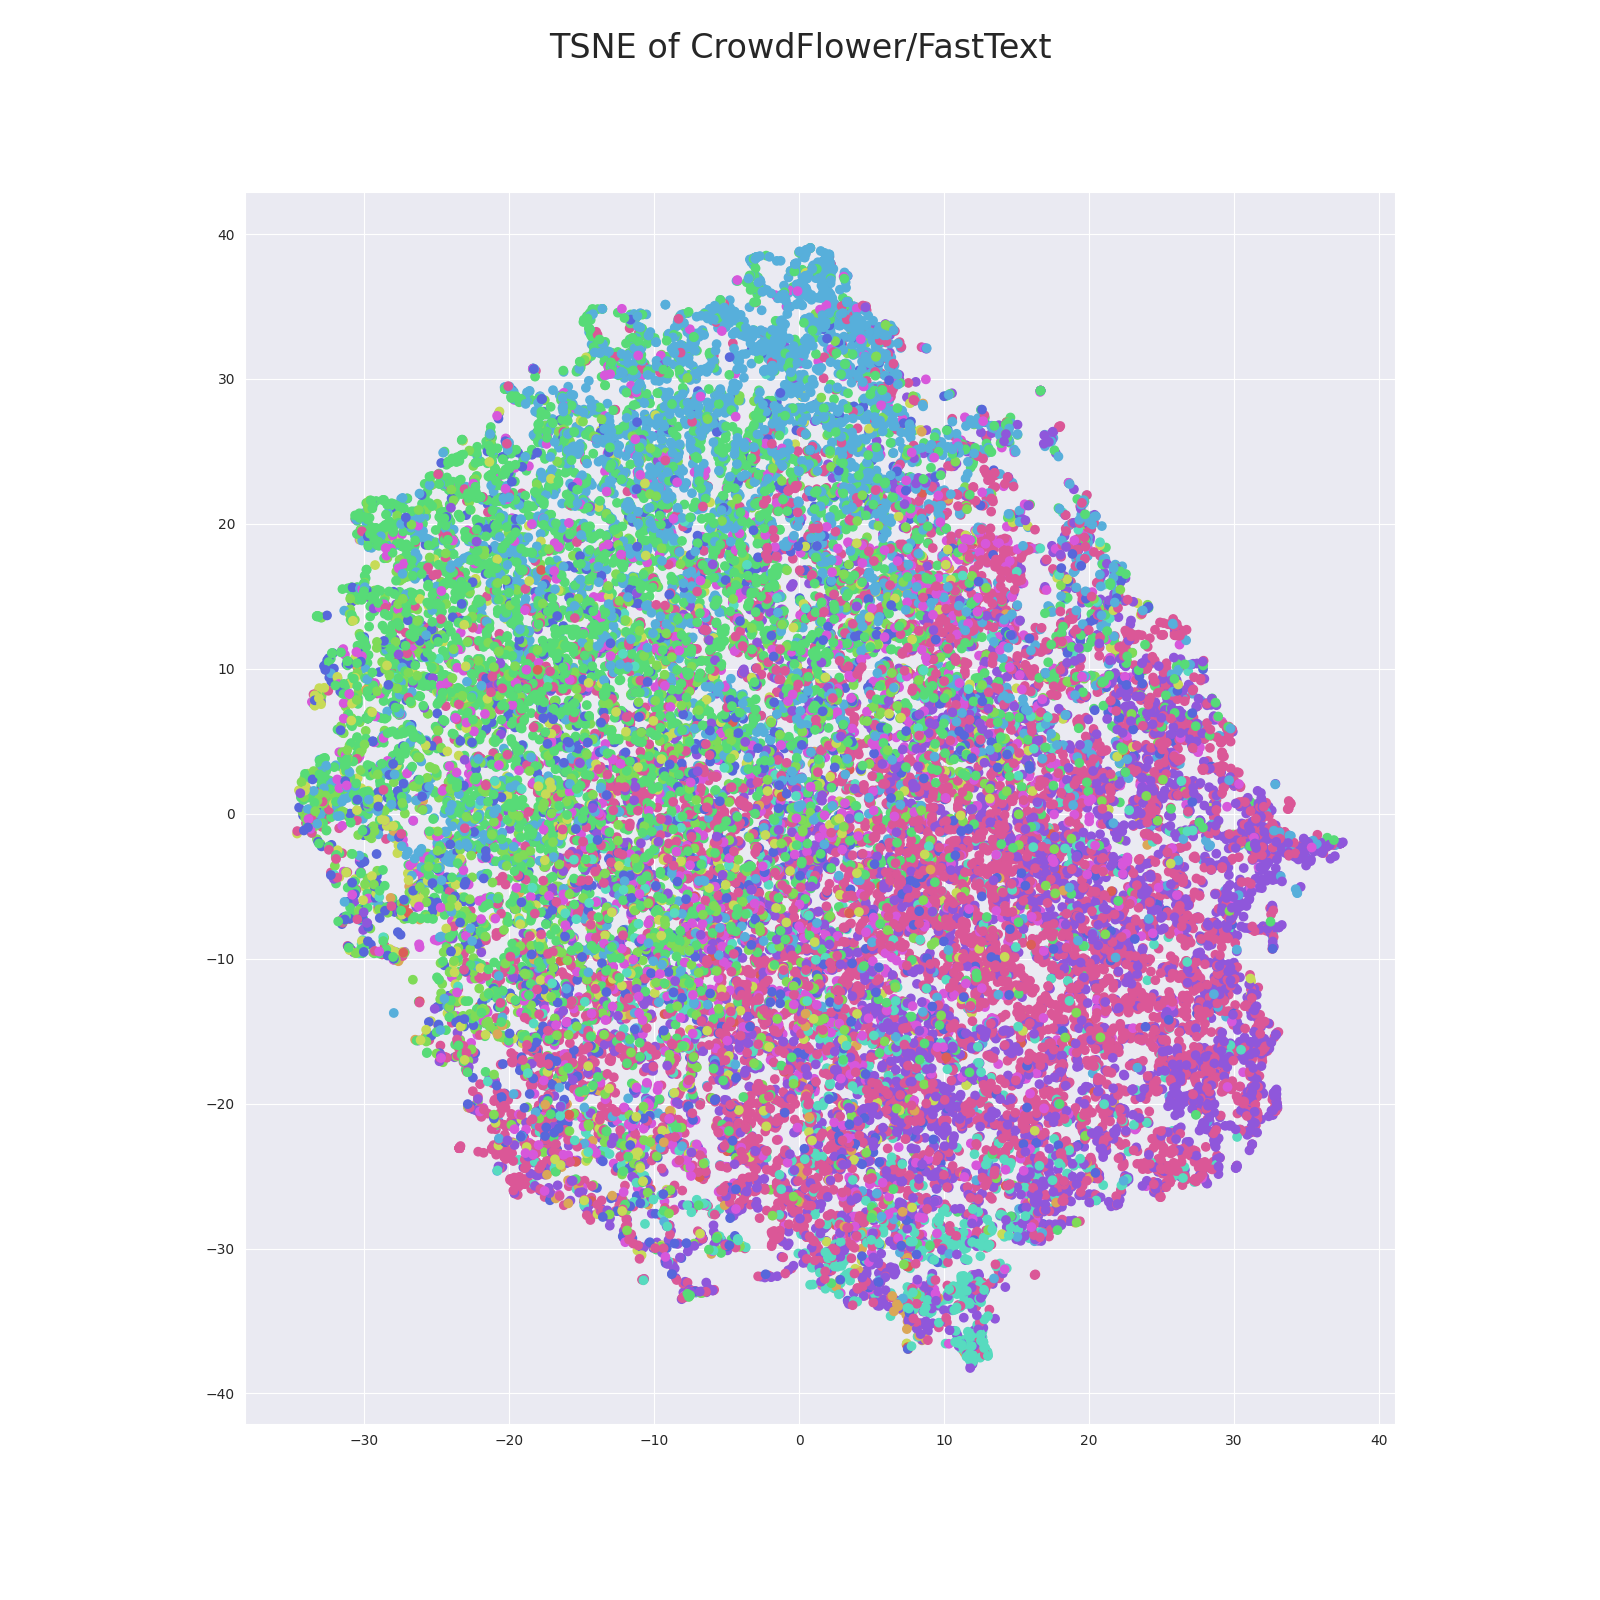
\includegraphics[width=1\textwidth]{plots/tsne/scat_CrowdFlower_FastText}
  \centering
  \caption{Scatter plot for TSNE of FastText}
\end{figure}\label{fig:scat_CrowdFlower_FastText}
It can be observed that Figure~\ref{fig:scat_CrowdFlower_FastText} shows clear gradients between groups. These are not linearly separable, but do comply with the emotion's valence value. Positive valenced emotions like Love, Fun and Happiness are present in the top part of the visualization (the positive side of component 1), while the negative emotions like Anger, Hate, and Sadness are presented in the lower part of the visualization. There is no clear separation of groups around the origin.
\subsubsection{Word2Vec}
As expected, the Word2Vec scatterinng does not present such clear groups as the ones shown by the FastText model. There is a main group of datapoints that fall around the origin, and a very slight gradient with positive valence at the bottom of component1, and negative valence at the top.
\begin{figure}[H]
  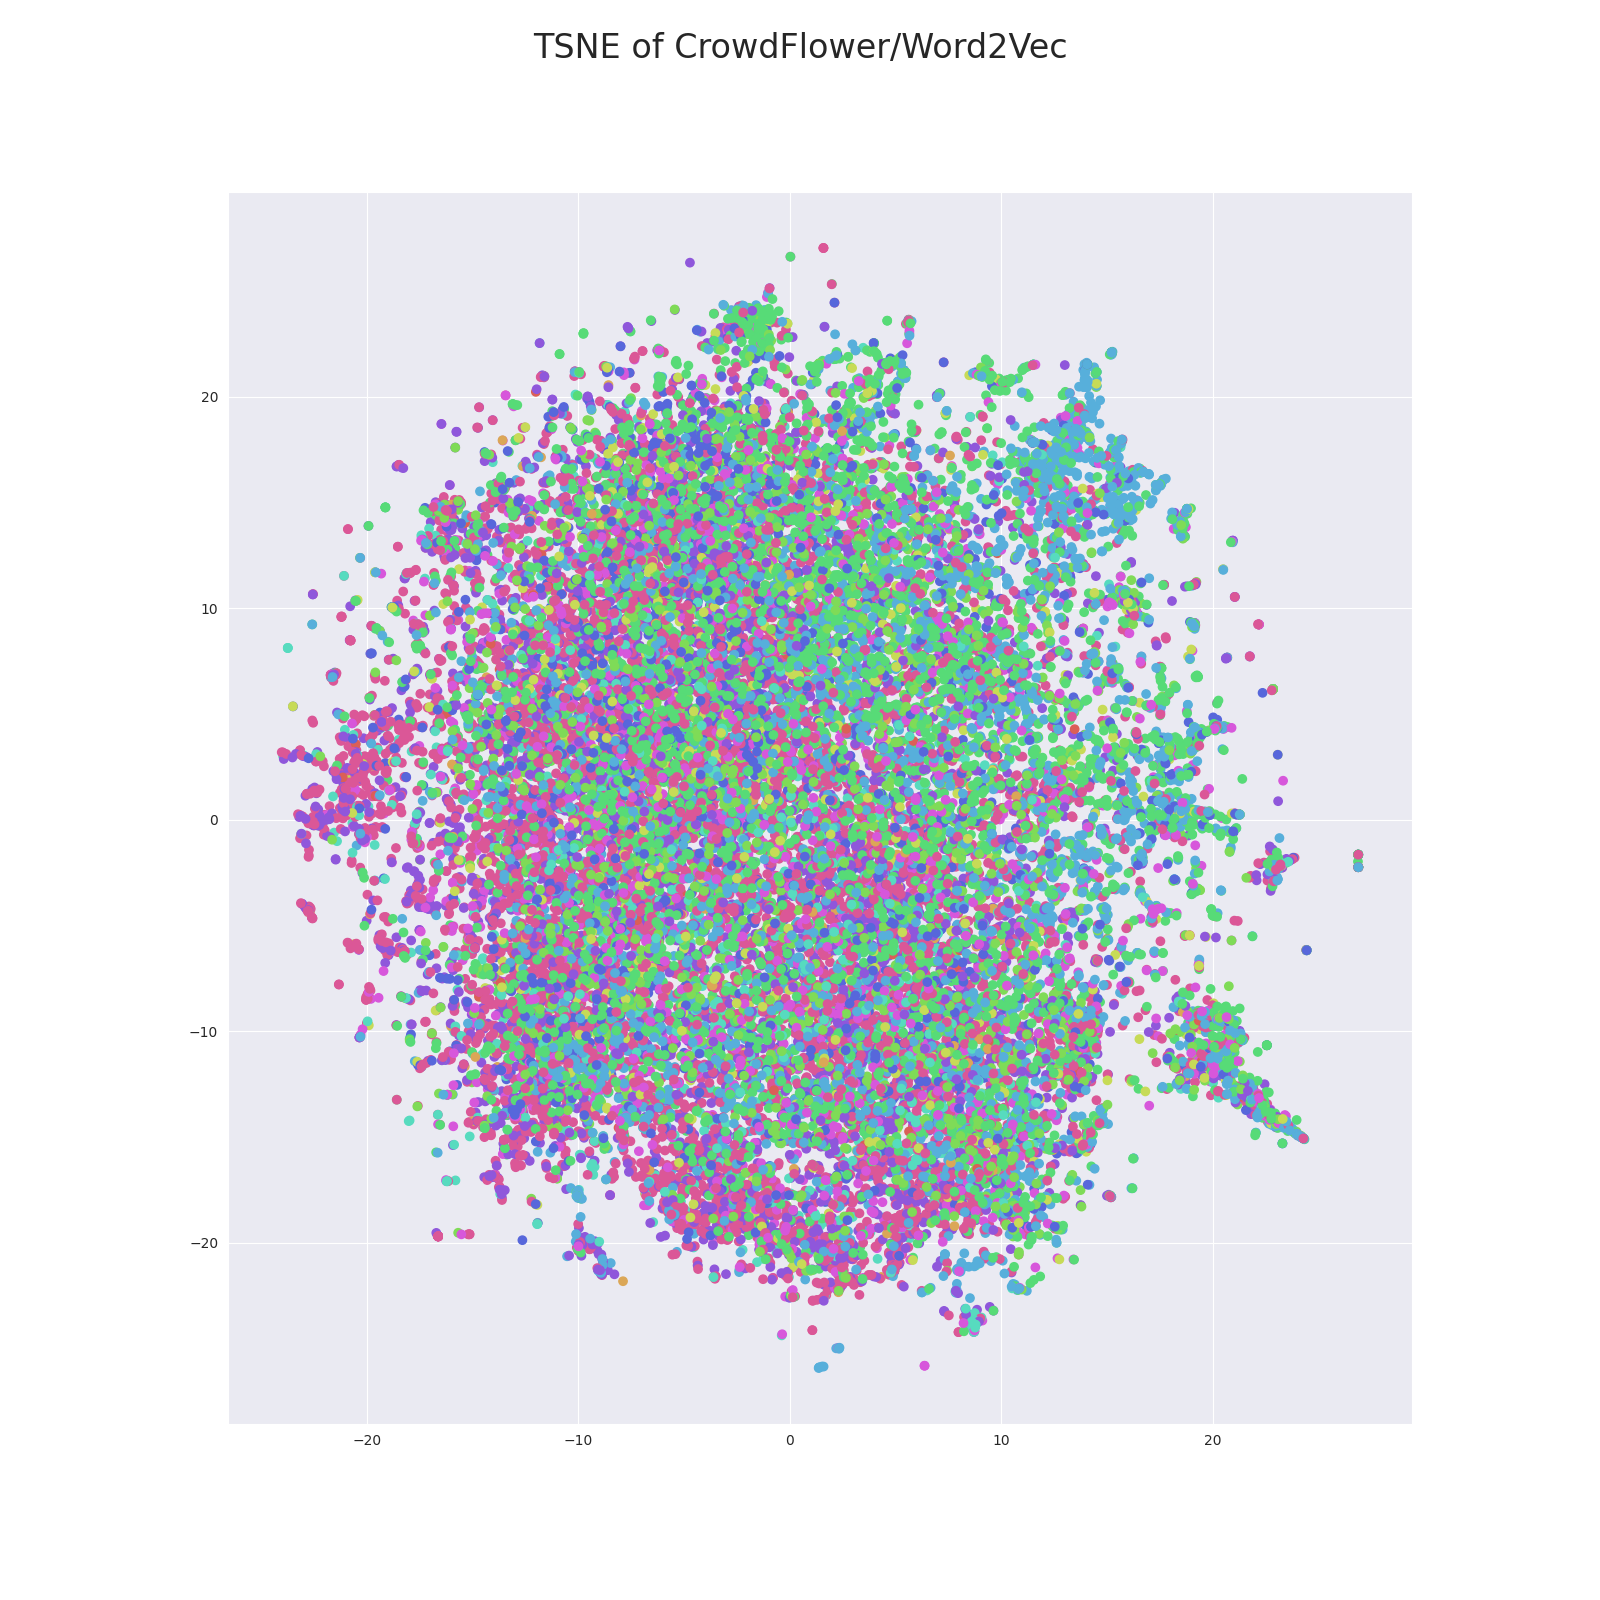
\includegraphics[width=1\textwidth]{plots/tsne/scat_CrowdFlower_Word2Vec}
  \centering
  \caption{Scatter plot for TSNE of Word2Vec}
\end{figure}\label{fig:scat_CrowdFlower_Word2Vec}
Figure~\ref{fig:scat_CrowdFlower_Word2Vec} shows a phenomenon present in pre-trained models. Some data points are separated from the main cluster, but are maintained relatively close to each other. These are sentences that are similiar in meaning, sometimes even identical sentences, but contain a distict emotional meaning.
% TODO: talk about the may4
\subsubsection{GloVe}
For the GloVe model, the gradient of positive and negative valenced emotions is not as clear as with the Word2Vec model.
\begin{figure}[H]
  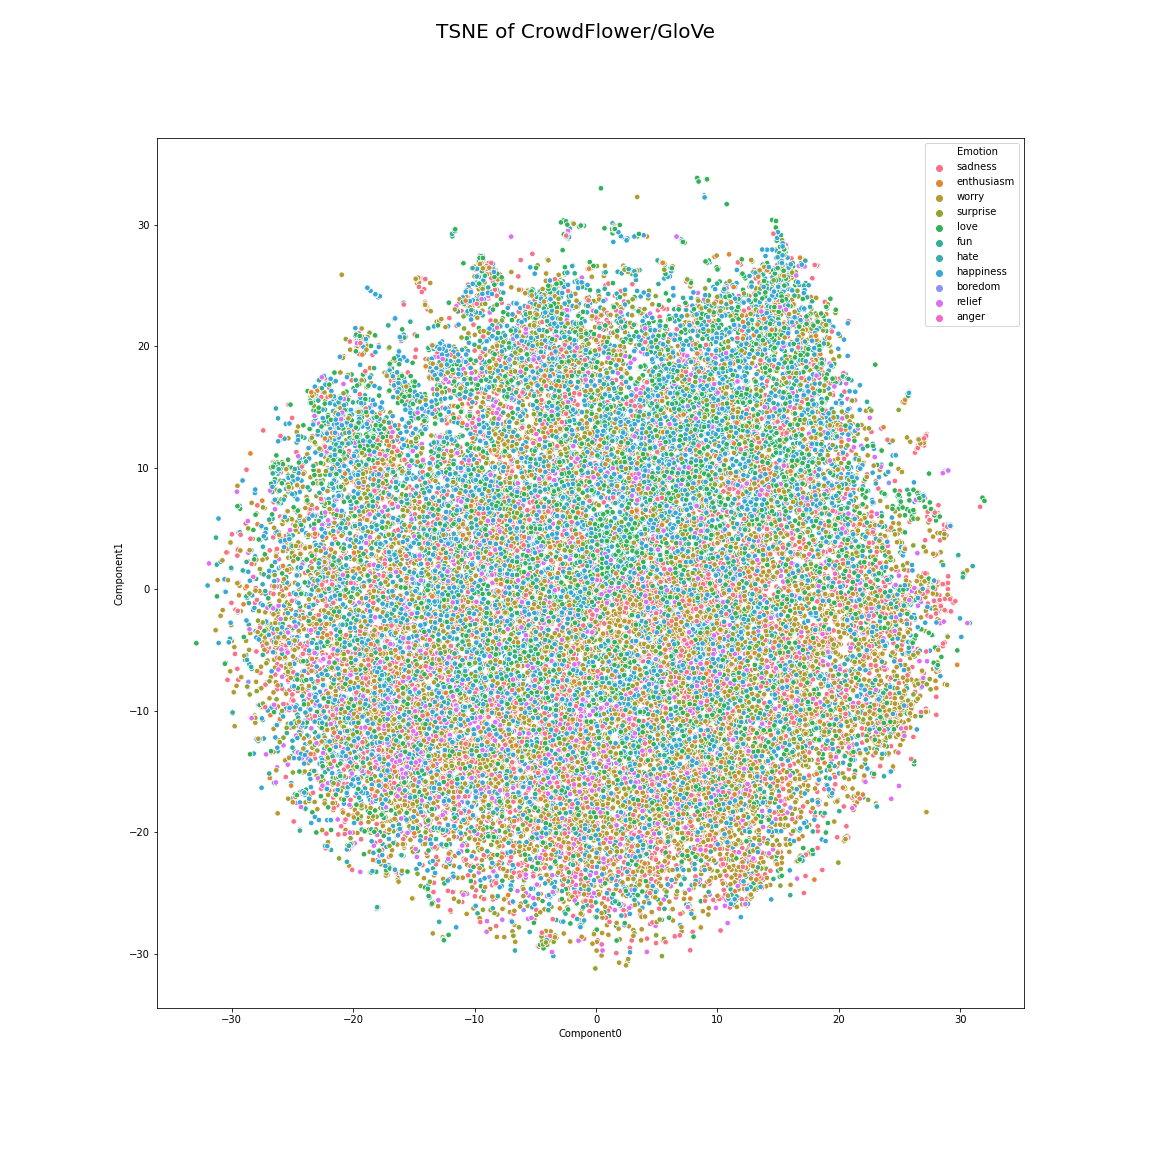
\includegraphics[width=1\textwidth]{plots/tsne/scat_CrowdFlower_GloVe}
  \centering
  \caption{Scatter plot for TSNE of GloVe}
\end{figure}\label{fig:scat_CrowdFlower_GloVe}
On Figure~\ref{fig:scat_CrowdFlower_GloVe} the dataset is represented mostly as a gaussian distribution of scattered datapoints. If there are relevant features of this representation, they are on the top of the visualization, where most of the positively valenced emotions are. There, the semantic clusters, seem to be more common than anywhere else in the plot.

\subsubsection{BERT}
With this analysis, BERT comes out as the model that creates representations that are linearly separable, even after using average representation of sentences.
\begin{figure}[H]
  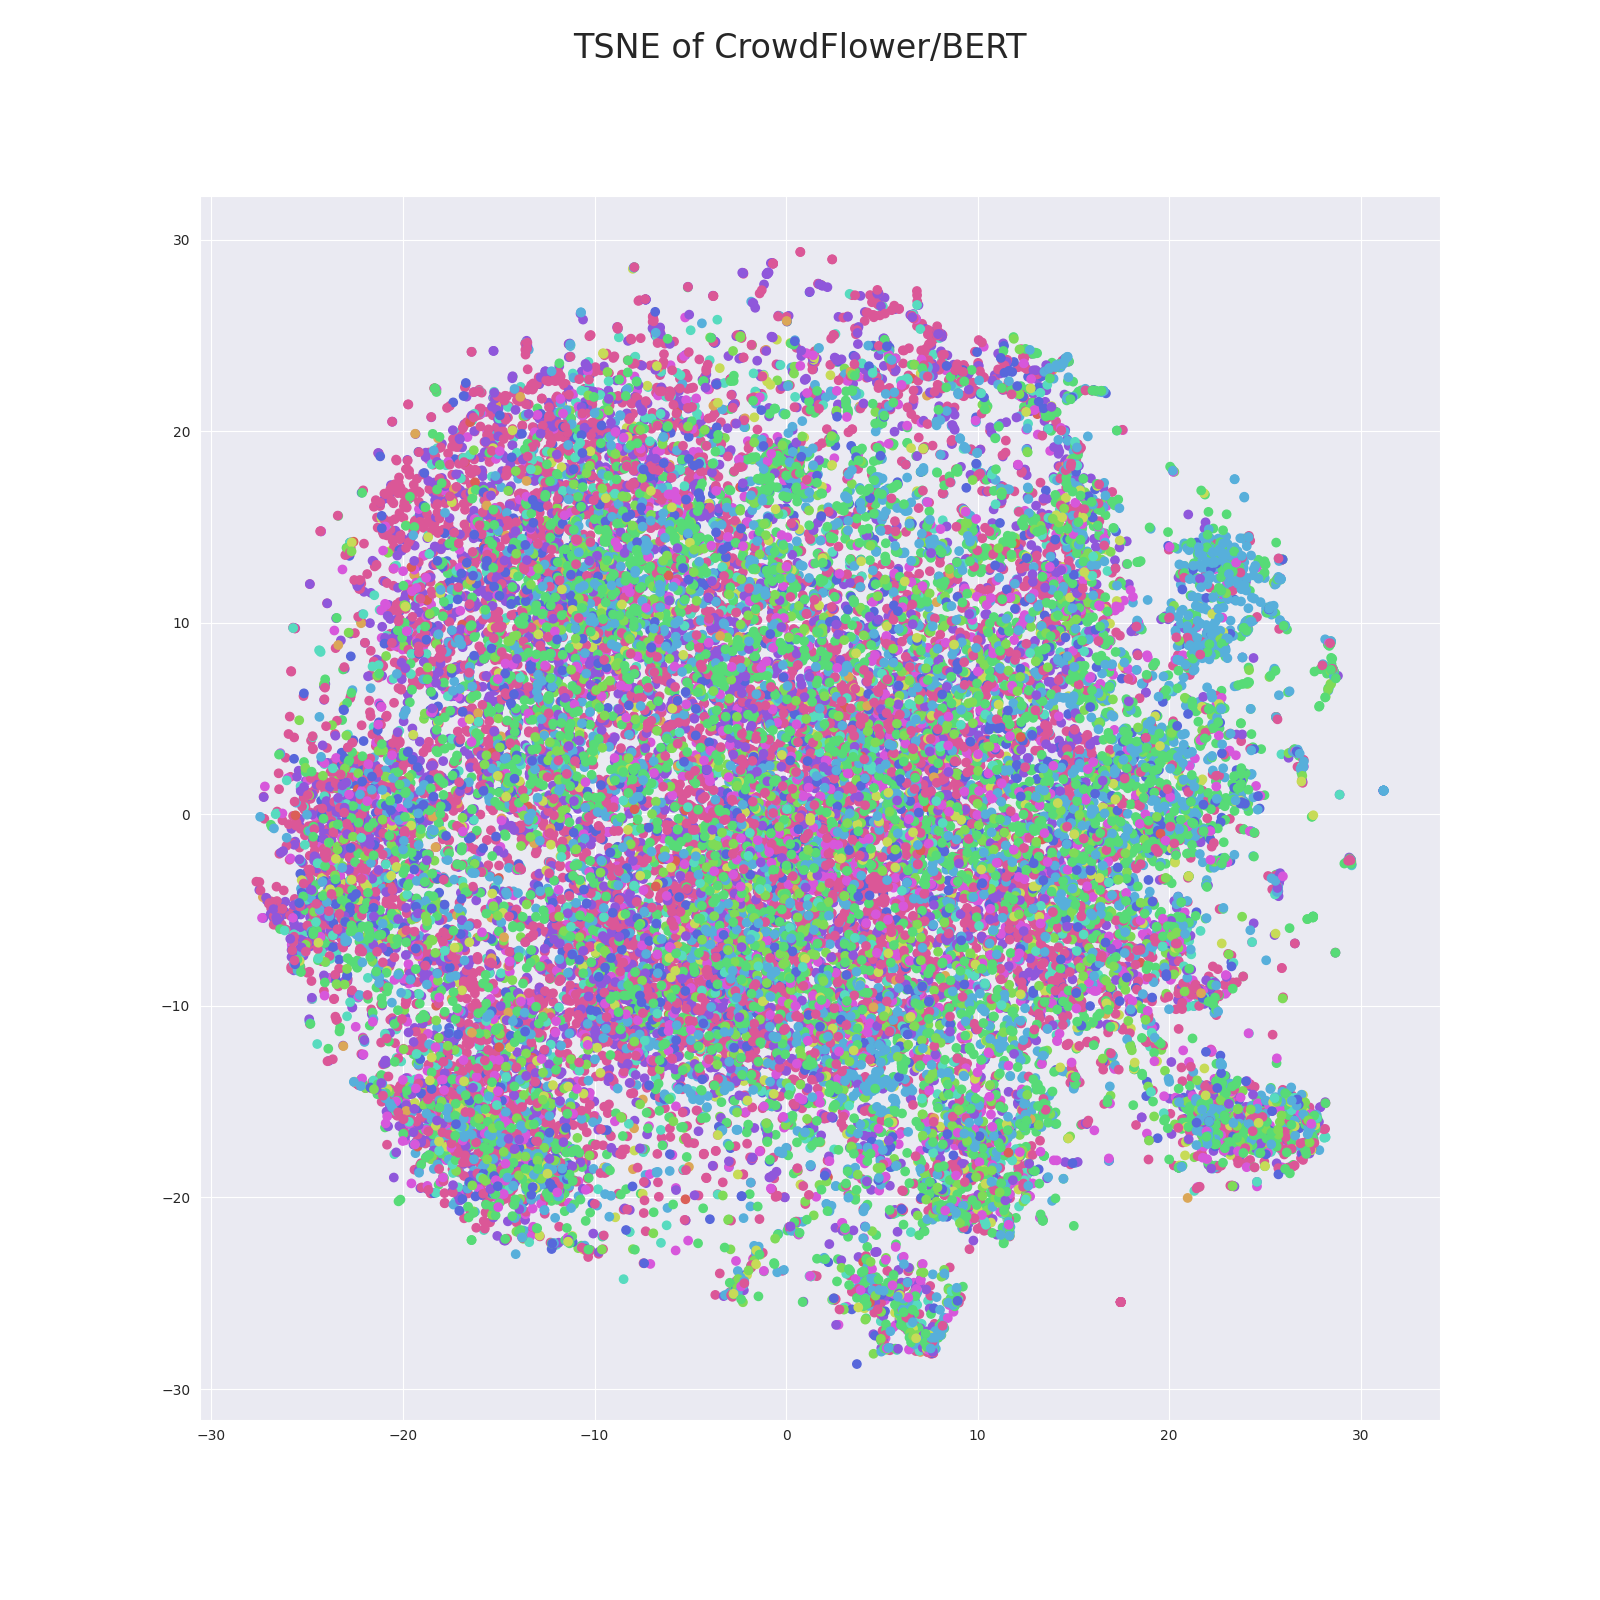
\includegraphics[width=1\textwidth]{plots/tsne/scat_CrowdFlower_BERT}
  \centering
  \caption{Scatter plot for TSNE of BERT}
\end{figure}\label{fig:scat_CrowdFlower_BERT}
In Figure~\ref{fig:scat_CrowdFlower_BERT} several clusters can be observed, with a very characteristiic one composed of mostly Love, Fun, and Happiness labels around (-17, -12). This cluster can be considered as a positive valence cluster. Although there are several groupings of sentences, there seems to be no clear gradient of valence in the model, but valence might be a variable to be measured inside clusters of datapoints.

\subsubsection{Analysis Discussion}
All models presented in this project are created through non-linear methods. The pre-trained models are also optimized to be used with neural networks. For this reason, a non linear approach is expected to yield the best result for a classifier.

%===============================================================================
\subsection{Result Analysis}\label{sub:Result Analysis}
The models presented here seem to have very little representation of emotions, but a strong relationship with valence. Although this could indicate that the models for human language do not conceptualize emotions, some cases have been found, that might indicate that it is in fact, the dataset that makes it difficult to cluster the conceptualization of certain emotions.
% TODO:
N of those cases are presented next.

\subsubsection{Class unbalance}
The class distribution of the CrowdFlower dataset is severely unbalanced. Table~\ref{tab:CrowdFlower_distribution} shows the classes, including neutral, which has been removed from this analysis.

\begin{table}
    \centering
    \begin{tabular}{|l|l|}
    \hline
      neutral     &  16894 \\
      worry       &  16840 \\
      happiness   &  10336 \\
      sadness     &  10284 \\
      love        &   7610 \\
      surprise    &   4360 \\
      fun         &   3532 \\
      relief      &   3042 \\
      hate        &   2640 \\
      empty       &   1606 \\
      enthusiasm  &   1510 \\
      boredom     &    358 \\
      anger       &    212 \\
    \end{tabular}
    \caption{Class distribution for CrowdFlower dataset.}\label{tab:CrowdFlower_distribution}
\end{table}

For this reason, the majority of the datapoints visualized in this project are Worry, Happiness, and Sadness.

\subsubsection{Semantic Clusters}
In the TSNE visualizations it's hard to pin down which datapoints represent what. For this reason, interactive visualizations have been made to explore freely the 2D space generated by this trasformation. This visualizations can be found in the project repository. By examining these visualizations several observations can be made.

The first one is that the models abstract semantics pretty well, as expected. Creating semantic clusters, or \"Meaning Islands\" for sentences that express the same idea, even if it's with different words. That's the case of the Star Wars island. This is a cluster in the Word2Vec TSNE transformation that clusters tweets sent on May 4th. (\textbf{Note}: the model did not have access to the date of the tweet, May the 4th is considered Star Wars day by the franchise's Fanbase) This cluster has a center around (26, -5). Tweets from this cluster include text like \"Happy Star Wars Day! May the 4th be with you\", \"Happy Star Wars day!\", or simply \"May the 4th be with you!\". Other tweets nearby include mentions of Bank's day, National days, or Fight Club's 10th aniversary.

Another interesting feature of this model is the \"ALL-CAPS\" peninsula on Figure~\ref{fig:CapsPeninsula}, on the other side of the plot, at around (-25, 11). This feature's most compact cluster are tweets of people whishing a happy mother's day, but also features some tweets cursing (with and without mentioning of mothers in the cursing), whishing happy birth day, and one about Star Wars day. All these tweets have in common that at least some part of it is written in all capital letters.

\begin{figure}[H]
  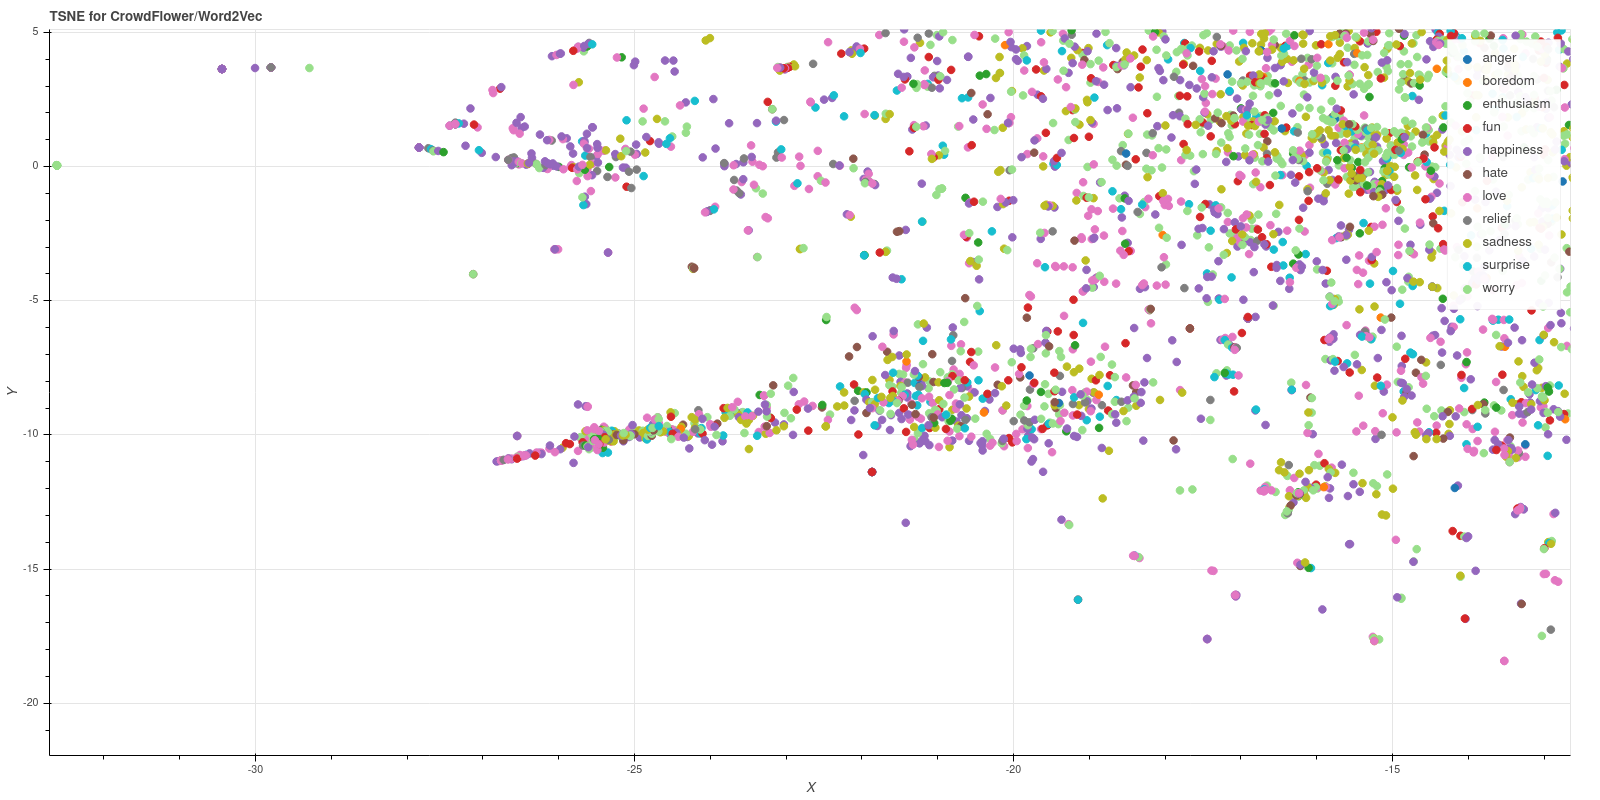
\includegraphics[width=1\textwidth]{plots/CapsPeninsula}
  \centering
  \caption{A zoom into the All-Caps peninsula for the TSNE transformation of the CrowdFlower DS under the Word2Vec LM}
\end{figure}\label{fig:CapsPeninsula}

Other interesting cluster is around (24, -10) in the Word2Vec projection, where most of the tags contain the word Happy, but are tagged with the emotion love.

In the GloVe projection, most tweets whishing for a happy mother's day seem to be disperese on the top region of the plot, but do not generally cluster.

A consecuent observation of these clusters is that very similar tweets have different emotional labels. This does not necesarily mean that the labels are wrong. But it does speak about the meaning that that tweet had for the person that asigned the label. Emotions are acording to theory, context dependant. Tweets for Mother's day are labeled with the emotions Love, Happiness, Fun, and even Wory.

A third observation comes from examining the dataset's text, where some of them are not in english. Some others are just links. In general there is an overload of people whishinig a happy mother's day and a happy Star Wars day. Both of these dates happen in May.

\subsubsection{FastText Approach}
The FastText Language Model, trained with this dataset, seems to have taken the three most frequent labels, and separated them to two different extremes of the vector space. This is exactly what a spervised model should do, but by doing so it sacrifices the clustering between sentences that might be related, but writen in a different manner.
